\documentclass[a4paper,12pt]{article}

\usepackage[left=3.5cm,top=2.5cm,right=2.5cm,bottom=2.5cm,includehead,includefoot]{geometry}

\usepackage{cmap}
\usepackage[T2A]{fontenc}
\usepackage[utf8]{inputenc}
\usepackage[russian]{babel}
\usepackage[pdftex]{graphicx}
\usepackage{color}
\usepackage{ulem}
\usepackage{amsmath}
\usepackage{xcolor}
\usepackage{longtable}
\usepackage{hyperref}
\usepackage{import}
\usepackage{bytefield}
\usepackage{datetime}
\usepackage{float}
\usepackage{dirtree}
\usepackage{colortbl}
\usepackage{url}

\graphicspath{{FIGURE/}}



\title{\Huge\textbf{Спецификация на ядро UART}}
\author{\huge RB}
\date{\today}

\pdfinfo{%
  /Title    (Спецификация на ядро UART)
  /Author   (RB)
  /Creator  (RB)
  /Producer (RB)
  /Subject  (IP-core specification)
  /Keywords (SystemVerilog, FPGA, UART, IP-core)
}


\begin{document}
\maketitle
\newpage


%
% --Список фигур---
%
\listoffigures
\addcontentsline{toc}{chapter}{\listfigurename}
\newpage

% --Список таблиц---
%
\listoftables
\addcontentsline{toc}{chapter}{\listtablename}
\newpage


%
%---Chapters----
%
%
% Introduction
%
\section{Введение}
\label{sec:introduction}

Данная спецификация описывает ядро UART, управление которым осуществляется при помощи интерфейса Avalon-MM или, в перспективе, AXI Lite (на данный момент находится в стадии разработки).

    \subsection{Интеграция}
    Изначально ядро предполагает интеграцию в QSYS САПР Quartus, но никто не запрещает добавлять его в любой RTL-код. Пример интеграции показан на рисунке \ref{img:integrated_ip}

    \begin{figure}[H]
        \centering
        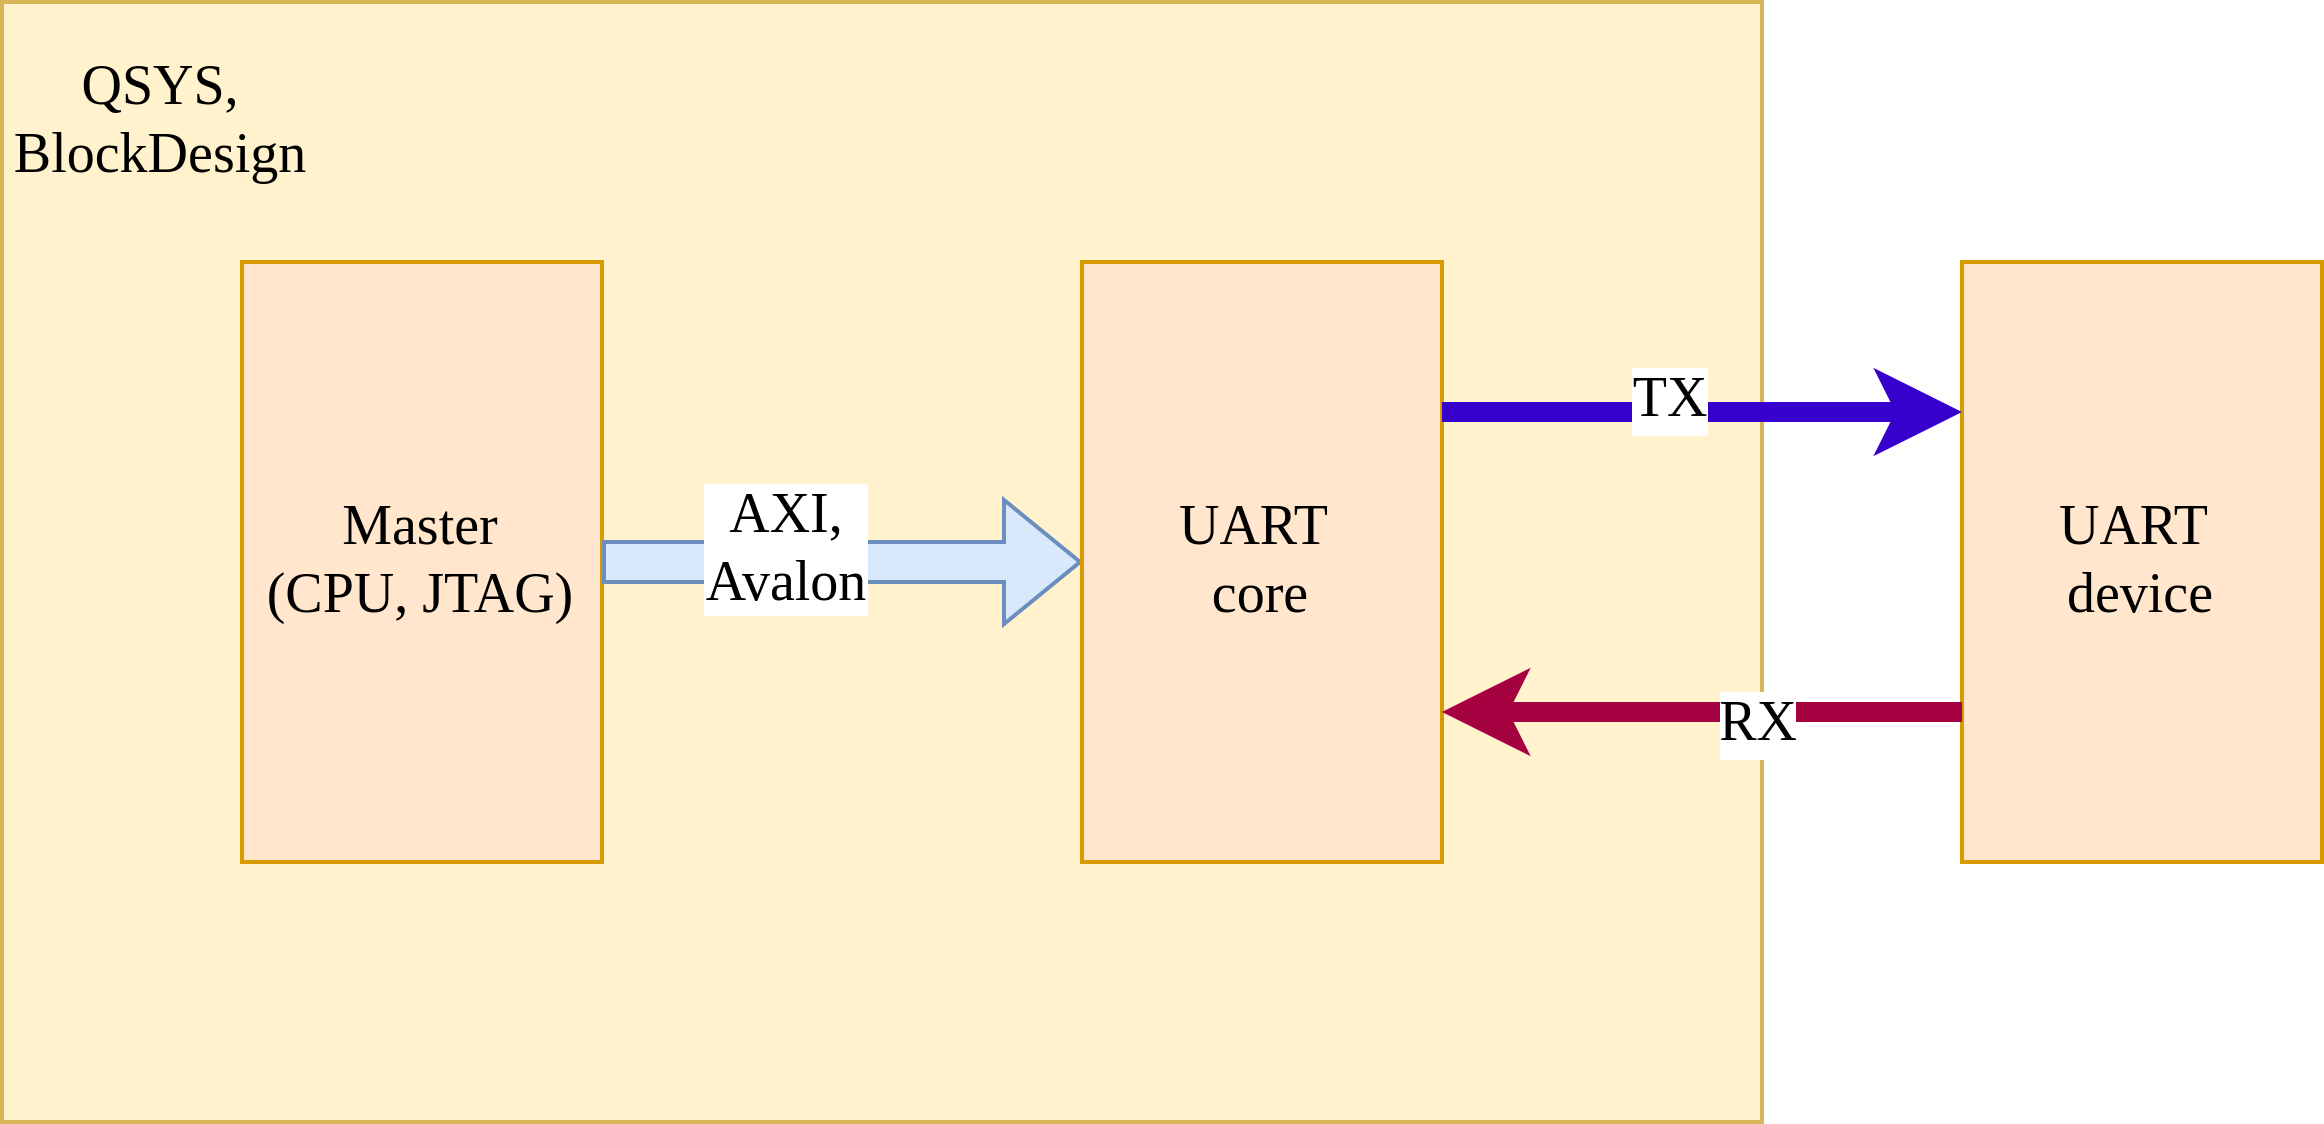
\includegraphics[width=11cm]{Integrate.png}
        \caption{Пример интеграции ядра в SoC}
        \label{img:integrated_ip}
    \end{figure}

    \subsection{Возможности ядра}
    Данное ядро обладает следующими возможностями:
    \begin{itemize}
     \item поддержка интерфейсов Avalon-MM и AXI Lite;
     \item программная установка любого BaudRate, в том числе не из таблицы стандартных скоростей;
     \item программное включение бита четности;
     \item поддержка odd и even битов четности;
     \item возможность установки до четырех стоп-битов
     \item настраиваемый размер приемного и передающего буферов.
    \end{itemize}



\section{Использование}
\subsubsection{Структура директорий}
  Проект содержит имеет следующую структуру папок:

    \dirtree{%
        .1 ..
        .2 RTL.
        .2 SIM.
        .2 OTHER.
        .2 DOC.
        .3 FIGURE.
    }

\begin{description}
    \item[\texttt{RTL}] - исходники ядра на языках Verilog и SystemVerilog,
    \item[\texttt{SIM}] - файлы для симуляции. \textbf{uart\_mm\_top\_tb.sv} - тестбенч для симуляции всего ядра. Для него предназначен \textbf{uart\_mm\_top\_wave.do} - скрипт для инициализации окна \textbf{wave} в \textbf{ModelSim/QuestaSim}). \textbf{uart\_tb.sv} - тестбенч для симуляции только приемопередатчика (проверка битов четности, стоп-битов и т.д.). Для него предназначен \textbf{wave.do} - скрипт для инициализации окна \textbf{wave} в \textbf{ModelSim/QuestaSim})
    \item[\texttt{OTHER}] - для прочих файлов,
    \item[\texttt{DOC}] - документация на ядро. Исходники в формате \LaTeX,
    \item[\texttt{DOC/FIGURE}] - хранилище изображений.
\end{description}










\end{document}
